% ********* 中文 ********%%%
% 第4章 设计
\section{Design}

% URN的设计目标是为提供一个统一的RDMA虚拟化框架,以适应混合虚拟化环境,同时实现统一的灵活的RDMA资源管理,并具备与原生RDMA接近的性能。此外,URN应尽可能确保最大的兼容性,对已有RDMA应用透明。
The goals of URN are: 1) to provide a unified RDMA virtualization framework for the hybrid virtualization environment where VMs and containers may be deployed on the same host machine; 2) to provide a single point of RDMA resource management for all RDMA resource users; 3) to keep the performance overhead of the RDMA virtualization to the minimum. Besides, URN should bring minimum impact to existing RDMA software stack and be completely transparent to the RDMA application. 

%URN主要包含了vRNIC,URN core和mgmt center。vRNIC是对虚拟机和容器通用的虚拟RDMA网卡设备,URN core则是各主机服务器上的用于集中管理RDMA资源的虚拟化层, mgmt center可以跨多主机管理协调RDMA网络的控制策略。在本章,我们介绍了URN中的一些关键性设计工作。
URN consists of 3 major parts, the vRNICs, the URN core and the management center. vRNIC is a virtual RDMA network device that looks like a real RDMA device inside VMs and containers. URN Core is a virtualization layer for centralized RDMA resource management on the host machine. And the management center is a centralized management entity in the data center keeps and coordinates management and control policies for the RDMA network.

% 4.1  vRNIC设计
\subsection{vRNIC}

% vRNIC是一个虚拟RDMA设备,由前后端驱动组成。后端在主机端,模拟RDMA设备;前端在guest端, 作为vRNIC的接口,转发guest应用的RDMA 命令到vRNIC后端。
The vRNIC is a virtual RDMA device that consists of a frontend and a backend. The vRNIC backend is placed in the host and emulates the behavior of a RDMA device. The vRNIC frontend is placed in the guest space that exposes RDMA device interfaces to the upper device drivers. Commands are forwarded from the vRNIC frontend to the vRNIC backend to be actually executed or emulated.

% 4.1.1 vRNIC后端
\subsubsection{vRNIC Backend}

% vRNIC后端被放在主机用户空间,因为vRNIC后端在用户空间有诸多好处,例如,更小的攻击面,更高的管理灵活性,以及对内核API无依赖等,具体细节可以见2.1节。
In URN design, the vRNIC backend is placed in the host user-space instead of the host kernel-space. This is because the device emulator in the user-space can be developed, deployed, managed more easily than that in the kernel-space. Also, its faults can be isolated from the OS kernel.

% vRNIC作为一个虚拟RDMA设备,vRNIC后端需要维护关于RDMA网卡的硬件属性,与物理RDMA网卡对应,例如RDMA地址vGID,RDMA设备类型等。此外,在vRNIC的运行过程中,vRNIC后端中需要维护三方面的上下文:
% 1,来自guest的虚拟RDMA上下文信息,主要记录了虚拟RDMA资源的信息;
% 2,由物理网卡创建的RDMA上下文,包含各RDMA资源,由vRNIC后端通过调用verbs库创建和维护;
% 3,虚拟RDMA上下文到物理RDMA上下文之间的对应关系。对应关系是一对一的,因为一对一是RDMA性能隔离的基础。
As a virtual RNIC device emulator, the vRNIC backend needs to maintain the same kinds of hardware properties that the physical RNIC has, such as the RDMA address GID, the RDMA device vendor. In addition, three kinds of contexts need to be maintained in the vRNIC backend at the run-time:
(1) Information of the runtime RDMA resources created and used on the emulated RDMA device, such as the memory address of the virtual MR/QP;
(2) Information of the runtime RDMA resources actually created and used on the physical RNIC,  such as the memory address of the real MR/QP;
(3) The mapping between the virtual RDMA context and the physical RDMA context.

% 如果guest中所有RDMA操作均转发到vRNIC后端执行,将会引入额外上下文切换及数据拷贝,例如,MR中的数据内容或QP中的工作请求等,从而导致RDMA性能下降。考虑到控制路径仅涉及到初始化和连接建立的过程,其开销是一次性的,而数据路径是影响RDMA性能的关键。因此,为了提高RDMA网络性能,guest中RDMA资源与vRNIC后端完成了映射,数据路径直接使用映射的RDMA资源,其命令未转发到vRNIC后端。具体来说,vRNIC后端与guest共享了一些内存区域,vRNIC后端使用该共享内存创建RDMA资源并映射给上层的guest应用,包括MR、QP、CQ和DoorBell等。然后,guest应用基于这些映射的RDMA资源执行数据路径的操作,这些操作会被RDMA物理网卡执行,不用经过vRNIC后端和虚拟机内核。因此,避免了额外的数据拷贝和进程切换,从而实现了与原生RDMA相当的性能。
When forwarding RDMA requests from the vRNIC frontend to the vRNIC backend, it causes context switching and data copying between the guest and the host. For example, when sending a data package, the data content in MR and the work request in QP need to be forwarded to the backend. This incurs performance degradation, especially on the data path. In order to achieve maximum performance, the RDMA resources are mapped in the shared memory region of the vRNIC backend and the RDMA application in the guest. On the data path, both the transmitted data and the sending/receiving requests are directly accessible to both the vRNIC backend and the RDMA applications, without an extra copy. Specifically, the vRNIC backend allocates RDMA resources in the shared memory region and RDMA the application in the guest maps to the same memory region in its own address space. The RDMA resources include MR, QP, CQ, and Doorbell. The RDMA application in the guest virtual environment puts data and requests in the shared RDMA memory region. The physical RNIC sees the data transmission requests in the shared memory region and performs the actual work without involving the vRNIC backend and the OS kernel in the guest virtual environment.

% 4.1.2 vRNIC前端
\subsubsection{vRNIC Frontend}

% 在虚拟机或容器中,vRNIC前端都是连接虚拟机或容器应用到vRNIC后端,但是它们的设计上有差别。 
% 在虚拟机场景中,vRNIC后端模拟了一个外部设备,由虚拟机OS中的vRNIC前端驱动。原生RDMA内核驱动包括与设备无关的OFED模块和设备相关的模块,OFED模块接收verbs操作并转化为内核层级的RDMA 命令;设备相关模块注册具体接口到OFED,并通过物理RNIC执行这些调用。对应的,在虚拟机中为了使用vRNIC,一个自定义的设备相关的驱动模块被构建在虚拟机内核,用来提供与原生类似的设备相关接口并注册它们到OFED模块。OFED中的RDMA命令将通过这些设备相关接口,被转发到vRNIC前端模块,再从前端转发到vRNIC后端去执行。因此,原生的RDMA应用无需修改便可运行在虚拟机中,而且虚拟机内核仍然可以使用RDMA。
% 在容器场景中,应用和vRNIC后端共享主机内核,仅位于不同的命名空间。为了在容器中使用vRNIC,容器的verbs库中与内核RDMA驱动交互的接口,被替换为vRNIC前端接口。Verbs操作被劫持到vRNIC前端,并被转发到vRNIC后端。
In both VMs and containers, the vRNIC frontend connects the application in the guest to the vRNIC backend, but the designs are different. In VMs, the vRNIC backend emulates as an external device, driven by the vRNIC frontend in the guest kernel. The native RDMA kernel driver includes device-independent modules (OFED) and device-specific driver. OFED accepts the Verbs operations and translates them into the kernel-level RDMA commands. The device-specific driver registers the specific interface into OFED and executes these calls via physical RNIC. Correspondingly, to use vRNIC in VMs, a custom device-specific driver is built to provide the similar device-specific interfaces and register them into OFED. But RDMA commands in the OFED will be forwarded to the vRNIC frontend via the registered device-specific interfaces; from there
they are further forwarded to the vRNIC backend to be executed. As a result, RDMA applications can run in the VM without modification, and RDMA can be used in the guest kernel. 

In containers, the application shares the host kernel with the vRNIC backend, only in different namespace. To use vRNIC in the containers, the Verbs library interfaces that interact with the RDMA kernel driver are replaced with the vRNIC frontend interface. The Verbs operations are hijacked to the vRNIC frontend and further forwarded to the vRNIC backend.

% 4.2  URN Core 设计
\subsection{URN Core}

% 为了对vRNIC进行统一管理,高效利用物理RDMA网卡,我们构建了一个统一的虚拟层URN core。URN core部署于集群的每台服务器上,监听虚拟机、容器以及原生的RDMA设备请求。之后,在URN core中实例化vRNIC和配置虚拟RDMA网络等。
To manage vRNICs uniformly and exploit the physical RNIC, we built a unified virtualization layer, namely URN Core. URN Core is deployed on each server in the cluster, listening for the request of RDMA device from VMs, containers and the native. After that, the vRNICs are instantiated and configurated with virtual RDMA network in the URN core.
%【 讨论:管理服务器的所有RDMA资源,对于来自虚拟机和容器的网卡资源申请,URN core会进行。1,发现和记录所有RDMA资源, 2,监控RDMA资源消耗,决策RDMA设备和资源分配(调度方式:动态轮询等等,调度目的:负载均衡、控制资源QoS),3,RDMA虚拟机容器的迁移信息】,

% 4.2.1 URN Core 服务
\subsubsection{URN Core Service}
% 【这段只有中文】URN core 服务会在每台服务器上运行,统一监听该主机上所有虚拟机、容器和原生的获取RDMA设备的请求(如果原生的请求不进行统一处理,将会导致原生和虚拟化对RDMA设备接口资源的冲突,因此修改了主机打开设备的Verbs实现,将对应请求转发到URN core,由URN core统一分配RDMA设备接口)。一旦有新的获取RDMA设备请求到来,便会唤醒URN core服务监听的描述符。URN core将开启新线程处理请求,并在请求处理完后结束线程。对于虚拟机和容器的申请vRNIC请求,URN core采用的是先来先服务的策略。如果需要区分请求的优先级,URN core中可以定义对应的优先级队列,再根据优先级处理请求。

% 4.2.1 实例化vRNIC 
\subsubsection{instantiating vRNICs}
% URN core在收到guest中应用申请vRNIC的请求后,会实例化vRNIC。实例化vRNIC的主要工作包括: 初始化vRNIC属性、绑定vRNIC到物理网卡、构建vRNIC前后端消息通道以及隔离各vRNIC实例等。
URN Core instantiates a vRNIC once receiving the request from the application in the guest. Instantiating vRNIC mainly includes: initializing vRNIC attributes, binding the vRNIC to the physical RNIC, building the message channel between the vRNIC frontend and backend, and isolating vRNIC instances.

% 初始化vRNIC属性:为了模拟与硬件一致的功能接口,URN Core需要对vRNIC的不变属性进行初始化,包括RDMA地址vGID,设备号等等。对于RDMA地址vGID,URN core会随机生成IPv6格式的虚拟值,同时登记到mgmt center的数据库中。
Initializing vRNIC attributes: To emulate the interface as physical RNIC, URN Core needs to initialize the invariant properties of vRNIC, including RDMA address vGID, device number, and so on. For RDMA addresses vGID, URN Core randomly generates the values in the IPv6 format and registers them into the database in the management center.

% 绑定vRNIC到物理网卡:vRNIC实例需要依靠物理网卡实现RDMA功能,因此,实例化vRNIC时需要将vRNIC实例与对应的物理RDMA网卡绑定。如果是多网卡设备或者多个网卡接口(如使用SR-IOV),还需确定从vRNIC到对应物理网卡接口的映射关系。
Binding vRNIC to the physical RNIC: The vRNIC instance relies on the physical RNIC to implement RDMA. Therefore, it is necessary to bind the vRNIC instance to the physical RNIC when instantiating. If there are multiple physical RNICs or interfaces (such as SR-IOV), the mapping from the vRNIC to the RNIC interface needs to be determined.

% 构建vRNIC消息通道:URN Core需要构建vRNIC后端与vRNIC前端之间的消息通道。对于容器来说,容器与vRNIC后端共享某一IPC命名空间,即可完成vRNIC前端与后端之间的消息交互。对于虚拟机来说,由于vRNIC后端在主机用户空间,而hypervisor位于主机内核空间。为了避免guest的消息先拷贝到hypervisor层再到vRNIC后端,我们构建一块共享内存,以此作为消息通道。具体来说,虚拟机物理内存与vRNIC后端之间是共享的。guest中的任意RDMA消息,均可以直接由vRNIC后端获取,同时也减少了从guest到vRNIC后端的延迟。
Build the vRNIC message channel: URN Core needs to build a message channel between the vRNIC backend and the frontend. For containers, the container can share an IPC namespace with the vRNIC backend to make the message interaction between the vRNIC frontend and the backend. For VMs, the vRNIC backend is in host user-space and the hypervisor is in host kernel-space. To avoid the messages being copied to the hypervisor and then copied to the vRNIC backend, we build a shared memory as the message channel. Specifically, the physical memory in the VM is shared with the vRNIC backend. Any RDMA messages in the guest can be fetched directly from the vRNIC backend, and the latency from the guest to the vRNIC backend is decreased.

% vRNIC实例隔离:URN core需要确保各vRNIC之间的消息通道是隔离的。在云环境中,同一主机上可能部署多个虚拟机或容器,该主机的URN core需要实例化多个vRNIC后端,以满足不同的guest实例。因此,需要确保各vRNIC之间的消息通道是隔离的,尤其是容器,由于其隔离性不如虚拟机彻底。如果多个容器和主机共享同一文件命名空间或IPC空间,那么,很容易通过扫描获取到其他容器或虚拟机vRNIC的消息通道。URN core利用了文件命名空间的机制,文件命名空间中的文件对于其他命名空间是不可见的。URN core在实例化vRNIC时,将各vRNIC消息通道对应的文件位于不同的命名空间,从而实现了各vRNIC实例之间消息通道的隔离。
RNIC instance isolation: URN Core needs to ensure that message channels between different vRNICs are isolated. In a cloud environment, multiple VMs or containers may be deployed on the same host, and the URN core of that host needs to instantiate multiple vRNICs for different guest instances. Therefore, you need to ensure that message channels between vRNICs are isolated, especially containers, which are not as completely isolated as VMs. If multiple containers and hosts share the same file namespace or IPC space, then it is easy to scan for vRNIC message channels to other containers or VMs. URN Core takes advantage of the mechanism of file namespaces, where files are not visible to other namespaces. When instantiating a vRNIC, URN Core places the corresponding files of each vRNIC message channel in different namespaces, to realize the isolation of message channels between each vRNIC instance.

% 4.2.2 配置虚拟RDMA网络
\subsubsection{configuring the virtual RDMA network}

% URN core在实例化vRNIC后,需要对vRNIC的网络进行配置,包括虚拟RDMA地址配置以及虚拟RDMA路由配置。
After the instantiation of the vRNIC, the URN core needs to configure the vRNIC's network, including virtual RDMA address configuration and virtual RDMA routing configuration.
For virtual RDMA address configurations, the vGID assigned to the vRNIC by URN Core is a virtual value, independent of the physical RNIC, when it instantiates the vRNIC.

% 对于虚拟RDMA地址配置,URN core 在实例化vRNIC时, 给vRNIC配置的vGID是虚拟值,与物理网卡无关。

% 对于虚拟RDMA路由配置,每台主机的URN core中配置了虚拟RDMA网络路由规则。具体来说,URN core在实例化vRNIC时,还给每个vRNIC都配置了组ID,路由规则的定义形式为:{group ID1, group ID2, Policy}。例如,如图4所示,容器1和容器2的vrnic被配置到同一组中,因此允许创建RDMA连接。作为对比,容器1和虚拟机1属于不同的用户组,按路由规则无法建立RDMA连接。各虚拟实例之间建立RDMA连接的具体细节可以参考4.3.1。
For virtual RDMA routing configurations, virtual RDMA network routing rules are configured in the URN core at each host. In particular, URN Core also configures the group ID for each vRNIC when it instantiates the vRNIC. Routing rules are defined as {group ID1, group ID2, Policy}. For example, as shown in Figure 4, the vRNIC of container 1 and container 2 are configured into the same group, thus allowing RDMA connections to be created. As a contrast, container 1 and VM 1 belong to different user groups and cannot establish an RDMA connection according to routing rules. See 4.3.1 for details on establishing RDMA connections between virtual instances.

% RDMA网络与传统TCP不同,RDMA还支持单边操作。在guest应用的RDMA单边操作中,RDMA的工作请求中包含了远端的GVA及key,远端MR内存地址同样需要在RDMA用户态驱动中转换为远端vRNIC后端的HVA。为了便于远端地址的转换,我们在URN core中建立了一个分布式的Key-Value数据库,存储各节点注册MR的映射关系{key,gva, hva}。在guest应用执行单边操作时,将向URN core 中的分布式KV数据库查询,以获取远端MR的HVA,缓存到本地并在写入工作请求以前。
Unlike traditional TCP, RDMA networks also support one-side operations. The remote GVA and key is included in the one-side work request, and the GVA also needs to be translate to the remote HVA in the RDMA user-space. To facilitate the remote memory address translation, we set up a distributed key-value database in the URN core to store the mapping of registered MR {MR-KEY, GVA, HVA} for each host. When the application in the guest performs a one-side operation, it will query the distributed key-value database in the URN Core for the remote HVA of MR, and caches it locally before writing the work request.

% 总之,URN core中的虚拟网络配置是动态调整的,因此,容器和虚拟机迁移后无需更改物理网卡及交换机等硬件的网络配置,实现便携的虚拟机或容器迁移。基于URN core中的虚拟路由规则,可以支持云环境中的多租户隔离。而各URN core存储的MR地址映射关系,对单边操作给予了支持。
In summary, the virtual network configuration in the URN Core is dynamical, so it is unnecessary to change the network configuration of hardware such as the physical RNICs and switches to enable portable VM or container migration. Based on virtual routing rules in the URN Core, multi-tenant isolation in a cloud environment can be supported. The MR memory mapping is recorded at each URN core to support one-sided operations.

\begin{figure}[!ht]
	\centering
	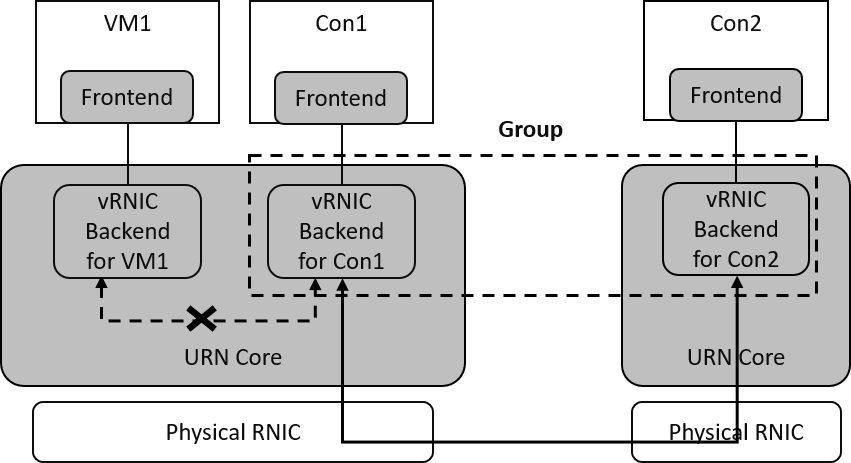
\includegraphics[width=1.0\linewidth]{images/route-config}
	\caption{Group Configuration and Routing: The vRNICs of container 1 and container 2 are configured in one group. Thus, two containers can create RDMA connections. And VM 1 are not allowed to create RDMA connections to containers in this figure because it is not added into the group. }
	\label{fig:route-config}
\end{figure}

% 4.3 Verbs库和用户态驱动 
\subsection{Verbs library and user-space driver}

%% 两小节: 控制路径和数据路径
%% 给图
% Verbs库为RDMA应用提供了统一的Verbs接口,在控制路径上,Verbs库接受RDMA应用的Verbs命令并与RDMA内核驱动进行交互,在数据路径上,Verbs库调用设备相关用户态驱动,绕过了操作系统内核。为了让虚拟机或容器中的应用使用vRNIC,同时确保URN对应用的透明性,Verbs库及其相关驱动需要适配vRNIC架构并提供与原生一致的Verbs接口。如图所示,针对控制路径和数据路径,在verbs库和用户驱动中有一些关键的修改工作。
The Verbs library provides the unified Verbs interface for RDMA applications. In the control path, the Verbs library forwards Verbs from RDMA applications to the RDMA kernel driver. In the data path, the Verbs library calls the device-specific user-space driver, which bypasses the kernel. To make URN transparent to applications, the Verbs library and driver to be adapted to the vRNIC while keeping the same Verbs interface as native RDMA. As shown in Figure~\ref{fig:verbs-driver}, there are key modifications in the Verbs library and user-space driver for both control path and data path.


\begin{figure}[!ht]
	\centering
	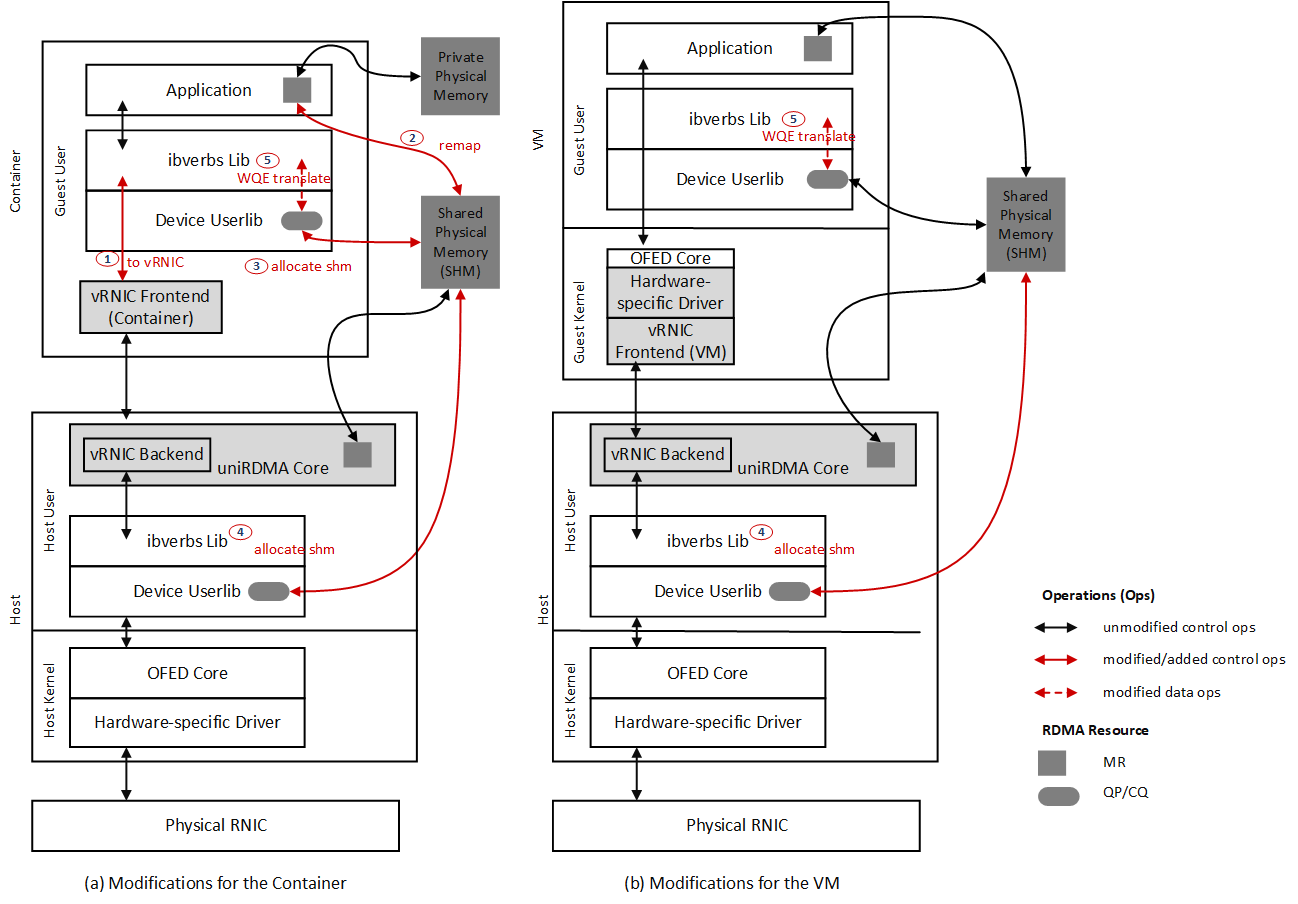
\includegraphics[width=1.0\linewidth]{images/verbs-driver}
	\caption{Main Modification in the Verbs library and User-space Driver for Containers and VMs}
	\label{fig:verbs-driver}
\end{figure}

% 在容器中,为了让Verbs转发到vRNIC后端,将Verbs库中到内核驱动的接口替换为到vRNIC前端交互的接口,如图4-a-1所示。此外,为了让容器应用与vRNIC后端之间完成RDMA资源的共享内存映射,包括MR、QP/CQ和DoorBell,具体修改如下:
%(1)针对MR:在原生RDMA中,MR的buffer是由应用指定的,并且通常是私有内存。在URN中,容器的Verbs用户库中将应用指定的MR内存重新映射到指定的共享内存,如图4-a-2所示。然后将该共享内存信息随Verbs命令及参数传递到vRNIC后端。vRNIC后端可以利用这一共享内存创建MR。
%(2)针对QP/CQ:原生RDMA中QP/CQ内存的分配是在用户态驱动中进行的,也不是共享内存。在URN中,我们在容器的用户态驱动中增加了分配共享内存作为QP/CQ buffer的函数(alloc_shm_buf,参加4.5节),如图4-a-3所示。对应的共享内存信息会随Verbs命令和参数传递到vRNIC后端。
% vRNIC后端在创建QP/CQ时,将分配这一共享内存作为QP/CQ的buffer。为此,我们增加了另一个新的函数(alloc_assigned_buf,参见4.5节),其指定具备特定地址的一块内存作为QP/CQ的buffer,如图4-a-4所示。
In the control path, there are different modifications between VMs and containers. In the container, to forward the Verbs calls to the vRNIC backend, the interface to the RDMA kernel driver in the Verbs library is replaced to the vRNIC frontend's, as shown in Figure~\ref{fig:verbs-driver} (a)-1. In addition, to achieve the shared memory mapping about RDMA resource between the application and the vRNIC backend, including MR, QP/CQ and Doorbell, there are more modifications in the Verbs library and user-space driver as follows:

(1) MR: In native RDMA, the MR buffer is assigned by the application and is generally private. In URN, the container's Verbs library will remap the GVA (guest virtual memory address) of the MR buffer to the shared physical memory, as shown in Figure~\ref{fig:verbs-driver} (a)-2. And the shared memory information will be forwarded to the vRNIC backend along with the Verbs call and parameters. The vRNIC backend can get the corresponding HVA (host virtual memory address) to register the MR, this operation is done by the vRNIC backend and out of the Verbs library.

(2) QP/CQ: In native RDMA, the QP/CQ buffer is allocated in user-space driver and not shared. In URN, we added a new API (alloc\_shm\_buf, see section 4.5) into the container's user-space driver to allocate the shared memory as QP/CQ buffer, as shown in Figure~\ref{fig:verbs-driver} (a)-3. The shared memory information will be also forwarded to the vRNIC backend along with the Verbs call and parameters. When the vRNIC backend creates QP/CQ, it will assign this shared memory as QP/CQ buffer. To achieve it, we add another new API (alloc\_assigned\_buf, see Section 4.5) in the user-space driver which assigns a memory piece with the specific address as QP/CQ buffer, as shown in Figure~\ref{fig:verbs-driver} (a)-4.

%(3)针对DoorBell:在原生RDMA中,verbs库打开RDMA设备接口,经RDMA内核驱动映射门铃到应用程序。在URN中,Verbs库打开虚拟的设备接口,并通过vRNIC后端和内核辅助模块来映射门铃。具体细节在第5节介绍。
(3) DoorBell: In native RDMA, the RDMA device is opened in the Verbs library and DoorBell is mapped to the applications through the RDMA kernel driver. In URN, the container's Verbs library opens the virtual device interface and maps the DoorBell through the vRNIC backend and a costumed kernel module. The details will be introduced in Section 5.

% 在虚拟机中,vRNIC在实例化时已经共享了虚拟机的整块物理内存空间。即使虚拟机应用使用默认的方式分配MR、QP或CQ等RDMA资源的内存,无需修改,vRNIC后端可以获取对应的共享内存块。具体地,通过虚拟机内核的vRNIC前端驱动中,将这些buffer的GPA(虚拟机物理内存信息)随RDMA命令和参数转发给vRNIC后端,vRNIC后端可以将GPA翻译为HVA,并使用这些共享内存块作为RDMA资源MR,QP或CQ的buffer,如图4-b-4所示。
In the VM, the whole physical memory of the VM is already shared with the vRNIC backend when the vRNIC instantiating. Though the application allocates the buffers MR, QP/CQ without modification, the vRNIC backend still can get the corresponding shared memory piece. In specific, through the vRNIC frontend in the guest kernel, the GPA (guest physical memory addresses of these buffers can be forwarded to the vRNIC backend along with the Verbs calls and parameters, and the vRNIC backend can translate the GPA to the HVA (host virtual memory address) and use the shared memory pieces as the buffers of MR, QP/CQ resources, as shown in Figure~\ref{fig:verbs-driver} (b)-4.

% 在数据路径上,针对虚拟机和容器场景的修改都一致。guest中未修改的RDMA应用往QP中写入工作请求,工作请求中待传输数据的内存地址仍然是GVA,RDMA物理网卡将根据缓存的页表检查工作请求中的地址,但是其缓存的MR页表信息则是主机vRNIC后端的HVA。因此,为了仍物理网卡成功执行guest中的工作请求,需要对RDMA工作请求中的GVA转换成HVA。为此,我们在guest用户态驱动中记录有MR资源的地址映射关系,即{key, GVA, HVA},在数据路径中,工作请求在写入QP之前,其gvm将转换成s-hvm。
In the data path, the modifications is same for VMs and containers. The unmodified application in the guest writes the QP buffer with a WQE (work request element) whose memory address for the transforming data is still the GVA, but the address will be checked in the physical RNIC through the cached page table that is about the HVA of the vRNIC backend. Therefore, to make the vRNIC execute the work request in the guest successfully, it is still necessary to convert the GVA to the HVA in the WQE, as shown in Figure~\ref{fig:verbs-driver} (a, b)-4. To achieve it, we record the memory address mapping relationship of MR buffer in the guest user-space driver \{MR-KEY, GVA, HVA\}, and the GVA of a WQE can be translated into the HVA before it is written into the QP buffer.

% 基于上述修改,无论是虚拟机还是容器,RDMA控制verbs将经过vRNIC前端到达vRNIC后端,在vRNIC后端中执行操作并映射RDMA资源。基于映射的RDMA资源,数据Verbs操作不需要转发到vRNIC后端,可以直接在guest用户空间,和原生RDMA一样避免了径额外的的拷贝或切换开销。
Based on the above modifications, in both VMs and containers, the control Verbs operations are forwarded into the vRNIC backend through the vRNIC frontend, the vRNIC backend executes the operations and map the buffers of RDMA resources. Based on mapped RDMA resources, the data Verbs operations are not forwarded to the vRNIC backend, and can executed directly in the guest user-space, which avoids the overhead of additional data copy or context switching as native RDMA.

% 4.3 虚拟RDMA workflow
\subsection{Virtual RDMA Workflow}
% 图4说明了虚拟RDMA的详细工作过程。虚拟RDMA的工作流程涉及guest中的应用、verbs库以及主机的vRNIC后端交互。整个工作流程依次分为初始化阶段、连接阶段和数据阶段。其中,初始化阶段分别包括设备打开和RDMA资源创建,连接阶段中RDMA应用通过QP与远端建立连接。数据阶段中RDMA应用执行数据路径的操作。
Figure 4 illustrate the detailed workflow of virtual RDMA. The workflow of the virtual RDMA involves the application, the Verbs libraries (including the user-space driver) in the guest, and the vRNIC backend in the host. In sequence, the whole workflow can be divided into initialization phase, connection phase and data phase. The initialization phase includes device opening and RDMA resource initialization. In the connection phase, the RDMA application establishes a connection with the remote through QP. In the data phase, the RDMA application performs the operations in the data path.

\begin{figure}[!ht]
	\centering
	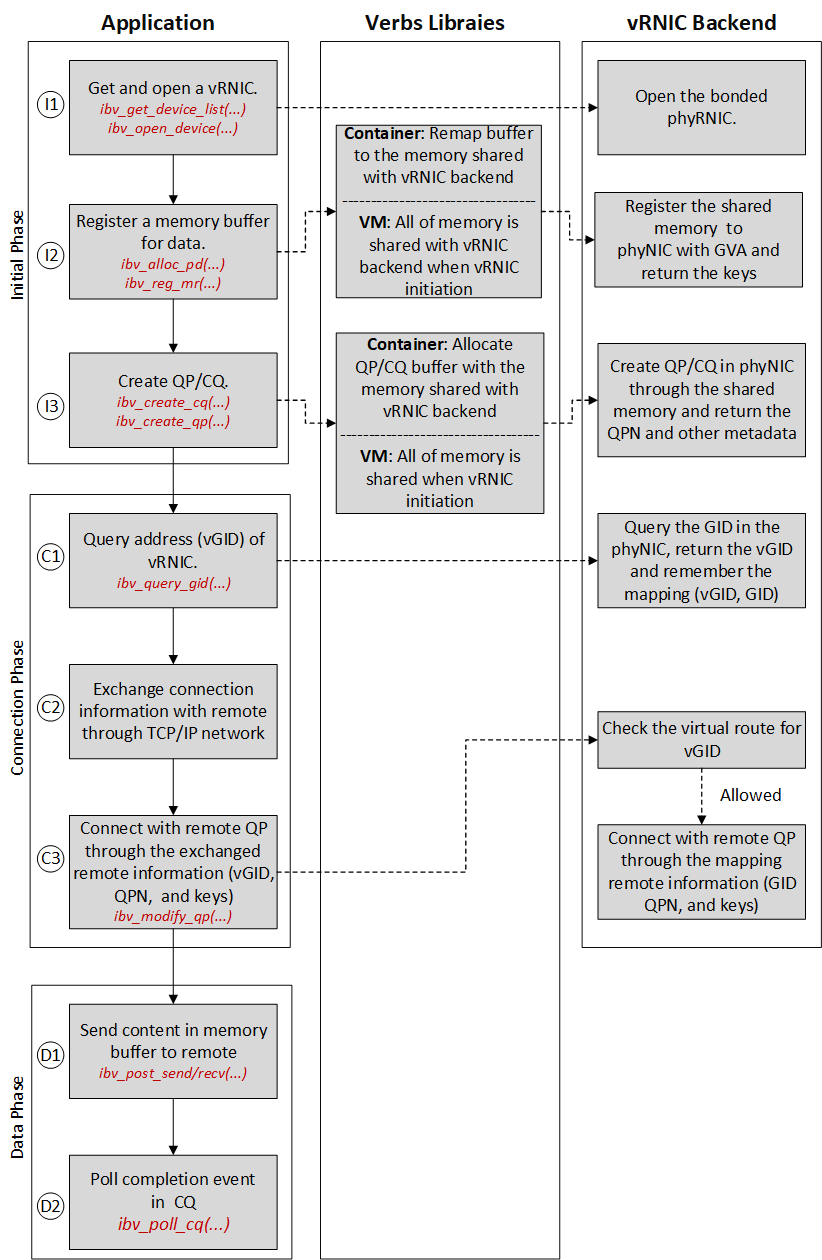
\includegraphics[width=1\linewidth]{images/RDMA-path.png}
	\caption{The Workflow of RDMA SEND operation}
	\label{fig:route-config}
\end{figure}

% 4.3.1 初始化阶段
%  初始化阶段主要完成资源的初始化,分别包括设备打开(I1)、注册内存buffer(I2)和创建QP/CQ等RDMA资源(I3)。具体细节如下: 
\subsubsection{Initialization Phase}
Initialization stage is mainly about the initialization of resources, including vRNIC device opening (I1), MR registration (I2) and QP/CQ creation (I3). The details are as follows:
% I1(Guest应用打开vRNIC设备):Guest应用依次调用Verbs接口ibv_get_devicelist和ibv_open_device,获取并打开vRNIC设备。这些调用会被劫持到vRNIC后端,vRNIC后端将打开在vRNIC实例化时绑定的物理RDMA设备。

I1(vRNIC Device Opening): The application gets and opens the vRNIC device by calling the Verbs ibv\_get\_device\_list and ibv\_open\_device in turn. The calls will be intercepted to the vRNIC backend, which will open the physical RNIC that was bound to the vRNIC when instantiation.

% I2(Guest应用注册MR):在容器中,Verbs库中将MR buffer重新映射到某一共享内存,虚拟机无需此步骤, 因为在实例化vRNIC时已与vRNIC后端共享整个内存。vRNIC后端会使用对应的共享内存注册MR,并返回MR buffer 的 HVM和MR-key等信息。在Verbs库中, 则会记录MR-key, GVA 和 HVA的对应关系,以用于后续的数据Verbs操作。
I2(MR Registration): In the container, the Verbs library remaps the MR buffer to a shared memory. This step is not required in the VM because the whole memory is already shared with the vRNIC backend when vRNIC instantiating. The vRNIC backend will use the corresponding shared memory to register MR, and return the HVM of MR buffer and MR-key, etc. In the Verbs library, the mapping {MR-KEY, HVA, GVA} is recorded for subsequent data Verbs operations.

% I3(Guest应用创建QP/CQ):在容器中,Verbs库使用共享内存分配QP/CQ buffer,虚拟机无需此步骤。vRNIC后端将创建QP/CQ时,使用对应的共享内存创建QP/CQ,并会返回QPN, CQN等元数据。 
I3(QP/CQ creation): In the container, the Verbs library use the shared memory to allocate QP/CQ buffer. The virtual machine does not need this step. The vRNIC backend will use the corresponding shared memory to create QP/CQ and return the metadata such as QPN, CQN.

%4.3.2 连接阶段
\subsubsection{Connection Phase}
% 连接阶段表示RDMA基于QP建立连接,依次包括查询GID(C1)、交换连接信息(C2)和基于QP建立连接(C3),具体细节如下:
The connection phase means that the RDMA connection is established based on QP, including querying GID (C1), exchanging connection information (C2) and establishing connection (C3) in sequence. The details are as follows:

% C1(获取GID):Guest应用调用Verbs ibv_query_gid,请求获取vRNIC的vGID地址。vRNIC后端将获取绑定的物理RDMA网卡的GID,记录(vGID,GID)对应关系, 并返回vGID给应用。 
C1 (Querying GID): The application calls Verbs ibv\_query\_gid for the vGID of vRNIC. The vRNIC backend will query the GID of the bounded physical RNIC, records the mapping {vGID, GID} and returns the vGID to the guest.

% C2(交换连接信息):应用与远端交换建立连接所需的信息vGID,QPN和MR key等。 该步骤完全由应用独立完成。例如,应用中可以使用TCP/IP 或RDMA-CM来交换信息。
C2 (Exchanging Connection Information): The applications exchanges the connection information with the remote, such as vGID, QPN and MR-KEY. This step is done independently in the application. For example, the application can use TCP/IP or RDMA-CM to exchange the information.

% C3(连接建立):应用调用verbs ibv_modify_qp 并将本地/远端的vGID、QPN等作为参数。该命令转发到vRNIC后端后,vRNIC后端会先根据URN core的路由表规则进行判断,如果允许,就会将本地/远端 vGID转换为对应的GID,再根据QPN,在两个vRNIC后端的QP间建立RDMA连接。
C3 (Connection Establish): The application calls the Verb ibv\_modify\_qp with the parameters, including local/remote vGID, local/remote QPN. The vRNIC backend will check the routing table from URN core. If allowed, the local/remote vGID will be converted to GID, and RDMA connection is established based on local/remote QP in two vRNIC backends through the QPN. 

% 4.3.3 数据阶段
% 数据路径发生在连接建立后,主要是对本地/远端 MR中的内容执行收发操作,包括图中的D1(收发数据)和D2 (轮询CQ)。具体如下:
\subsubsection{Data Phase}
The data phase is after the RDMA connection is established and about how to send/receive the content in the local/remote MR buffers, including D1 (Send/Recv Data) and D2 (Poll the CQ). The details are as follows:

% D1(收发数据):在双边操作中,两端应用分别执行Verbs ibv_post_recv和ibv_post_send对本地MR中的数据进行收发。对于其中的参数WQE, Verbs库会将其中的本地MR数据地址GVA转换为HVA。在单边操作中,仅执行ibv_post_send,但是WQE参数中包括了本地/远端 MR数据块地址。在第一次执行单边操作时,将向vRNIC后端获取远端MR GVA与HVA对应关系,并缓存到本地Verbs库,然后对本地/远端 MR数据块地址执行从GVA到HVA的转换。
D1 (Send/Recv Data): In two-side operation, data in the local MR can be sent and received by executing Verbs ibv\_post\_recv and ibv\_post\_send, respectively. For the parameter WQE, the Verbs libraries will translate the local MR data address from GVA to HVA. In one-sided operations, only ibv\_post\_send is called, but the parameter WQE includes the local/remote MR data address. When the first one-side operation, the mapping {GVA, HVA} for remote MR buffer will be queried from the vRNIC backend, cached into the Verbs libraries, and there the local/remote MR data address will be converted from GVA to HVA.

% D2(轮询CQ):Guest应用轮询CQ来获取对应的工作完成通知。如果使用事件通知机制,guest中verbs库将等待vRNIC后端获取事件并返回给应用。
D2 (Polling the CQ): The application poll the CQ for the work completions. If event-based notification is used, the Verbs libraries will wait for the vRNIC backend to receive the event and return it to the application.

% 4.4 mgmt center
\subsection{Management Center}

% 在URN框架里,整个集群配备一个mgmt center,作为配置管理策略,存储各节点RDMA资源信息的中心。

% 通过mgmt center,管理者向不同节点的URN core下发各种策略,包括控制平面策略,如连接管理,防火墙等;和数据平面策略,如Qos、流量计费等。管理框架图如图5所示:策略由mgmt center下发到URN core,URN core通过agent接收策略后,其中,URN core将控制平面策略配置给管理的各vRNIC后端。对于数据平面策略,URN core将其发送给各guest Verbs库中的agent,然后在各RDMA应用本地执行。

%  连接管理、防火墙等控制平面策略主要基于RDMA连接进行,而RDMA连接依靠QP等RDMA资源,因此,这些策略主要依靠RDMA资源,如QP进行控制。由于包括QP在内的所有RDMA资源均已经映射在vRNIC后端中,因此,控制策略可以直接传送到各vRNIC后端,依靠映射的RDMA资源执行。 对于数据路径,依靠监控各vRNIC后端维护的映射好的RDMA资源,如QP/CQ等,可以完成QoS等数据功能。然而,这样做将消耗额外的CPU资源而且对轮询的处理效率要求极高。因此,本文将数据策略进一步从URN core下发到各guest的用户库,在各RDMA应用本地执行,策略执行结果则可以返回给URN core或mgmt center。注意,这些扩展需要所有客户机都信任库,并且这些修改应该包含在TCB(可信计算库)中。对照native的RDMA,其数据路径绕过了操作系统内核,而RDMA物理网卡的数据管理功能及其有限,因此,其细粒度的数据管理同样需要由Verbs库配合执行。

\begin{figure}[!ht]
	\centering
	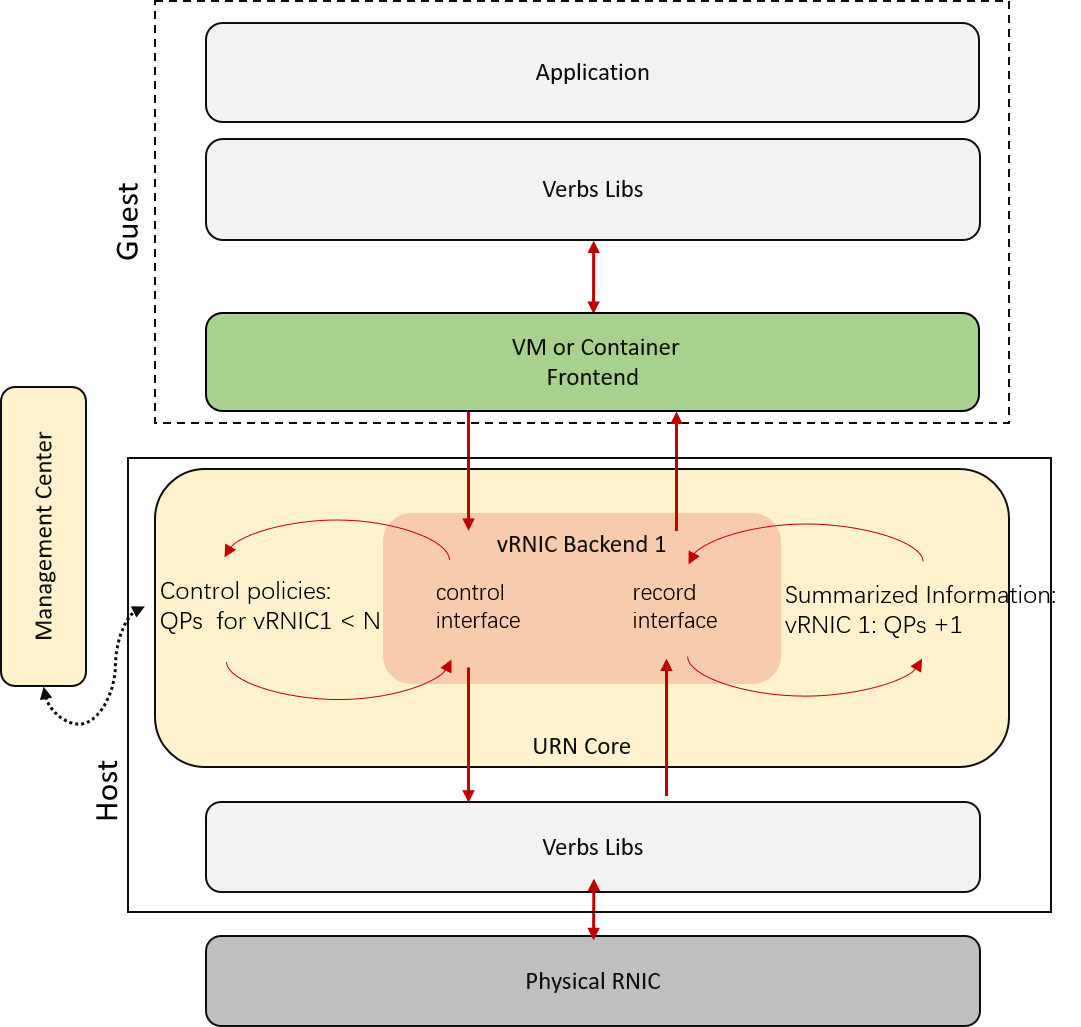
\includegraphics[width=1\linewidth]{images/urn-interface.png}
	\caption{The Architecture of URN Management}
	\label{fig:route-config}
\end{figure}

% 4.5 discussion
% 随着云计算环境的复杂化,不同的需求越来越多,对RDMA虚拟化提出了更多的要求。结合可能的需求,本节讨论了RDMA虚拟化可能面临的一些需求和解决思路:
\subsection{Discussion}

%  (1)虚拟机迁移: 容器或虚拟机迁移在云中有很多好处,例如资源利用和故障转移。迁移分为脱机迁移和动态迁移。在脱机迁移中,虚拟机或容器关机后,迁移到远端后重新启动。因为URN core维护了网络地址的映射关系,该关系可以直接发送给迁移后节点的URN core,无需修改guest 中RDMA应用内部的网络地址。对于动态迁移,一般都需要借助AccelNet方案【引用】,应用释放RDMA资源,使用TCP/IP网络完成迁移,然后显式地重新建立RDMA连接。对于这种方式,我们也可以无缝支持。
Virtual Instances Migration: Migration of containers or VMs has many benefits in clouds, e.g. resource utilization and fail-over. With the virtual RDMA network, URN can support offline migration without reconfiguring the physical RDMA network for applications. In specific, after rebooting the migrated virtual instance, the application can rebuild the RDMA connection through the same network address. The only work is modifying the address mapping in URN core. Currently, for live migrations, it is still hard because memory regions in RDMA application may be uncertain under bypassing or one-side communication. And the problem is unrelated to URN.

% (2)对RDMA虚拟化扩展的支持:RDMA虚拟化中,需要对QP/CQ等RDMA资源进行资源映射,避免额外的数据拷贝及切换开销。现有的Verbs库和用户态驱动没有对RDMA资源映射的支持。为此,我们建议Verbs库或设备相关库中增加以下API,以加强对各场景下RDMA虚拟化的支持,尤其是应用可以使用新增加的Verbs接口显式地完成MR、QP/CQ等资源的映射。如下表所示:
% API  所属库  功能 
% alloc_shm_buf()  设备相关库 创建并分组共享内存作为RDMA资源内存
% alloc_assigned_buf(addr, size) 设备相关库 为RDMA资源指定某一内存区域
% ibv_create_shm_qp/cq() 基于共享内存区域创建QP/CQ
% ibv_assigned_qp/cq 使用指定的内存区域创建QP/CQ
% ibv_reg_shm_mr() 使用共享内存区域注册MR

% 此外,为了实现高性能的数据传输,RDMA网卡缓存了应用注册内存的页表信息。在用户态虚拟化后,现有的RDMA网卡只能缓存虚拟层MR的页表信息,而无法缓存guest应用使用MR的页表信息。在URN的实现里面,尽管通过在URN core KV数据库和本地缓存数据库实现了高效的地址转换,但是引入了额外的工作量。因此,为了更好地适配虚拟化场景,建议Verbs库在创建MR时额外提供一个指定网卡缓存guest应用页表的地址参数,如原来的ibv_reg_mr(..., s-hva)扩展为ibv_reg_mr(..., s-hva, gva)。稍后,RDMA内核驱动可以根据新注入的gva参数,为该MR指定与guest应用对应的页表。

% (3)扩展虚拟Verbs接口: 目前我们设计Verbs库的主要考虑是与原生的Verbs库兼容,以实现对RDMA应用的透明性,但是,这样会导致容器应用只能基于URN verbs库使用虚拟RDMA,或者基于原生Verbs库使用RDMA,从而导致了使用RDMA的局限性。解决这一问题的可能思路是,扩展Verbs库,增加获取虚拟RDMA设备的专有Verbs接口,供应用选择调用。
%%%*********************%%%